

\section{\heiti 方法}
\subsection{\heiti 总体流程}


本研究提出的司法判决预测方法,其核心在于构建一个能有效整合案件事实、法律法规及类案判例的智能推理框架。整体流程如图\ref{fig:main}所示。
首先,系统接收待判决案件的详细事实描述($C$),并利用预训练的LLM进行初步语义分析和关键信息抽取。LLM从复杂的案情描述中识别并初步推断出罪名类别、犯罪构成要件(包括主体、主观、客体、客观)及证据特征等核心法律要素,形成结构化的犯罪核心要素表示($F$)。
其次,系统基于抽取的犯罪核心要素$F$,并行地从法律条文数据库和案例数据库中检索相关信息。
一方面,从权威的法律条文数据库中检索出与案件特征$F$高度相关的法律法规条款集合($L$)。另一方面,从海量的历史案例数据库中智能检索出与当前案件在罪名构成、事实情节和证据方面最为相似的判例集合($S$)。
最后,将原始案件事实描述$C$、初步提取的犯罪核心要素$F$、检索到的相关法律条文$L$以及筛选出的相似判例$S$作为共同的上下文信息,输入至LLM。LLM将进行综合分析与推理,输出最终的判决结果($J$)。

该模型作为核心推理引擎,通过整合这些多源异构信息,综合考量法律原则、司法解释及类案判例的指导作用。这不仅有效弥补了LLM在法律专业知识和复杂逻辑推理方面的固有局限性,而且显著增强了判决预测的专业性、准确性和可解释性。
\begin{figure*}[!htbp]
	\begin{minipage}{0.5\linewidth}
			\centering
	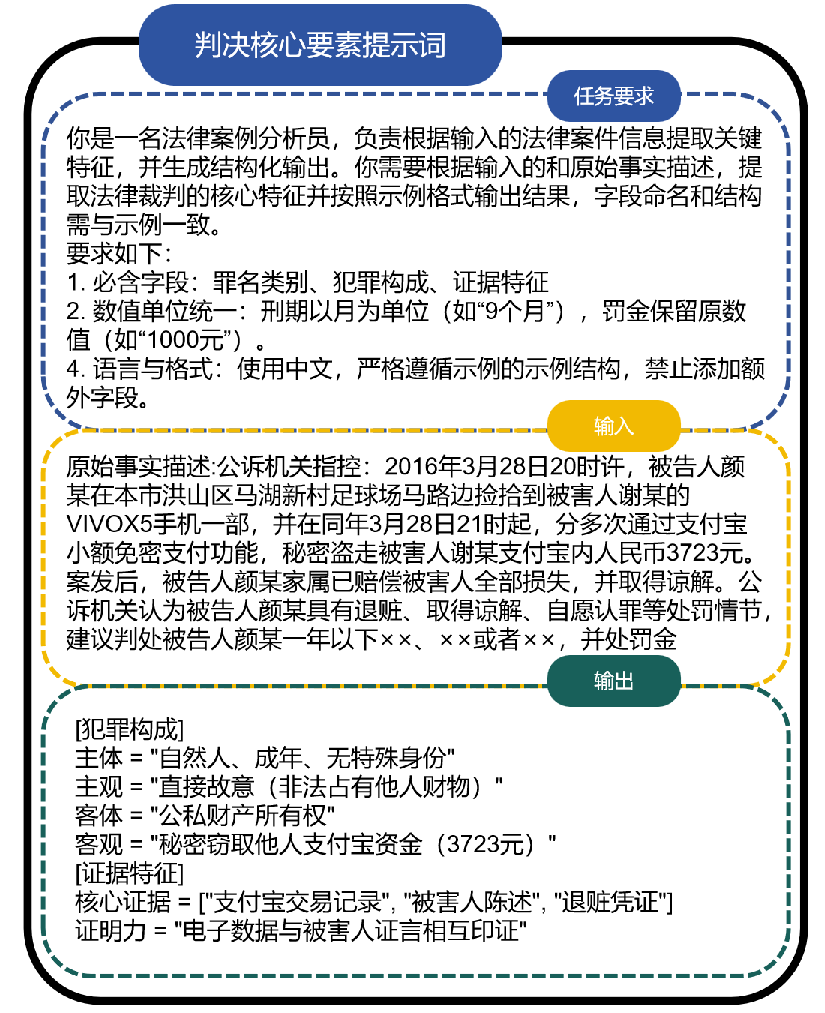
\includegraphics[width=1\linewidth]{fig/prompt1.pdf}
	\caption{判决核心要素提示词}
	\label{fig:prompt1}
	\end{minipage}
	\begin{minipage}{0.5\linewidth}
		\centering
	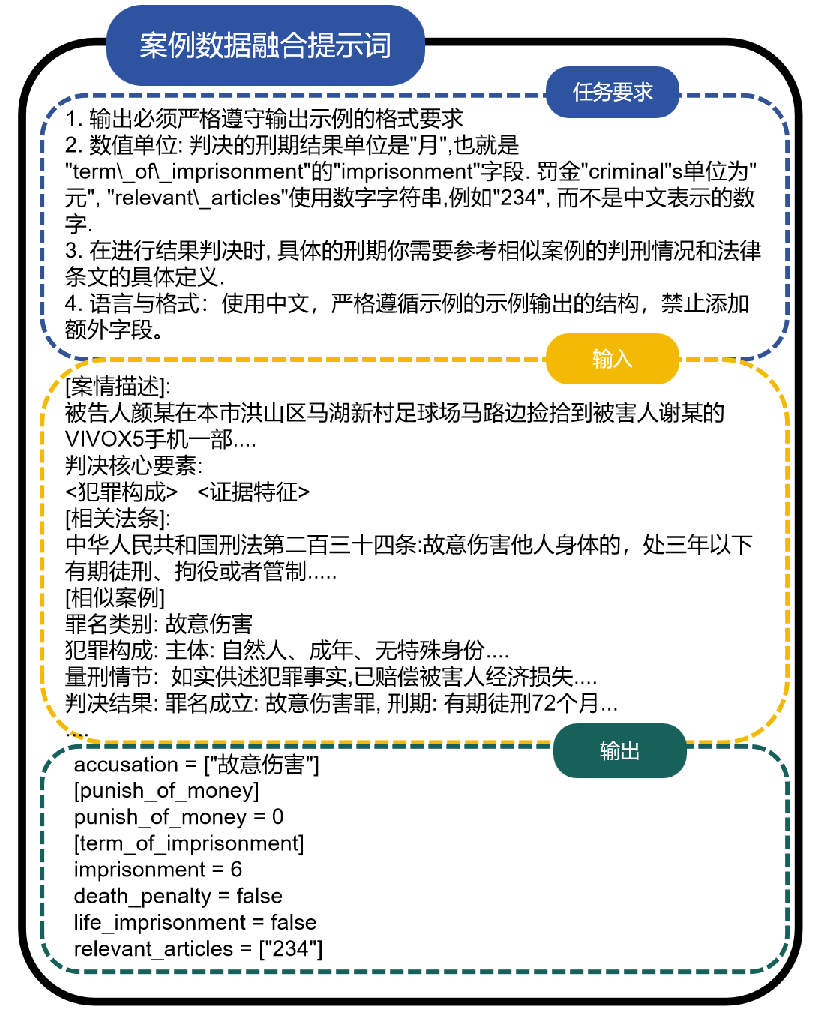
\includegraphics[width=1\linewidth]{fig/prompt2.pdf}
	\caption{案例数据融合提示词}
	\label{fig:prompt2}
	\end{minipage}
\end{figure*}


\subsection{\heiti 判决核心要素提取}
在大陆法系的刑法理论中,一项行为若要被判定为犯罪,其客观事实必须符合刑法分则具体条文所规定的全部构成要件。
此外,法官在进行司法判决时,还需要综合考量检察机关提供的证据、犯罪嫌疑人的行为动机以及造成的事实性后果等因素。
然而,传统方法未能识别法律要素间的逻辑依赖,导致判决预测缺乏法律推理的前提,最终可能造成判决结果不可信甚至错误~\cite{JSJA202505027,zhao2022charge,zhao2022charge}。
为解决此问题,本研究提出了判决核心要素提取方法。判决核心要素$F$由犯罪核心要素和证据核心要素构成。其中,犯罪核心要素包括犯罪主体、犯罪客体、犯罪主观和犯罪客观四个方面。证据核心要素由证据和证明力组成。证据指检察机关提供的直接证据,而证明力是证据的可信程度,表明证据之间相互印证、逻辑连贯,能够充分证明犯罪行为。该证据特征通过LLM定制提取。明确识别判决核心要素有助于去除冗余信息和噪声,为后续的法律条文检索与相似案例检索提供精确、简要的数据,并为逻辑关联分析和推理奠定基础。
\textit{判决核心要素提示词}从事实描述$C$中提取,其示例详见图\ref{fig:prompt1}所示。
明确提取犯罪核心要素和证据核心要素,不仅优化了案件结构化理解的基础,也为后续的法律条文检索和判决文本生成提供了更为精准和逻辑严谨的输入。这从而提升了整个智能判决系统的透明度、准确性以及与人类司法实践的一致性。

\subsection{\heiti 相关法律条文检索}
为解决LLM在法律知识方面的不足和潜在的“幻觉”问题,相关法律条文检索通过引入真实的法律条文,为LLM提供准确、权威的法律规范依据。这确保了模型在进行判决预测时,能够明确犯罪的构成要件、法律定义以及量刑的法定边界。首先,本研究构建了一个包含各类法律法规的法律条文数据库($DB_{law}$​​)。
数据库中的每条法律条文均通过文本嵌入模型转换为高维向量表示,并存储于向量数据库中,以支持高效检索。
当处理新案件时,从案件事实描述$C$中提取的犯罪核心要素$F$同样被转换为查询向量$F_e$​。
随后,系统采用近似最近邻搜索算法,通过计算查询向量与数据库中法律条文向量之间的相似度,检索出与案件最为相关的k条法律条文,形成集合L。
\begin{equation}
	\begin{aligned}
		L  =(l_1​,l_2​,\dots,l_k​)
		=\text{Topk}​(\text{Sim}(F_{e},DB_{law})),
	\end{aligned}
	\label{eq:L}
\end{equation}
其中,$\text{Topk}​$表示取相似度最高的$k$个结果,$\text{embed}$表示文本嵌入函数,$\text{Sim}$是相似度计算函数。


数据库中的每条法律条文均通过文本嵌入模型转换为高维向量表示,并存入向量数据库以支持高效检索。当处理新的案件时,从案件事实描述$C$中提取的犯罪核心要素$F$同样被转换为查询向量$F_{e}$。随后,系统采用近似最近邻搜索算法,通过计算查询向量与数据库中法律条文向量之间的相似度,检索出与案件最为相关的$k$条法律条文,形成集合$L$。该过程可表示为:

\subsection{\heiti 相似案例检索}
为解决仅凭法条和案例描述难以覆盖所有复杂情况,并促进“同案同判”的问题,本研究提出了相似案例检索方法。该方法旨在从历史判例中寻找与当前待审案件在核心特征上相似的案例,为LLM提供司法实践层面的参考。
相似案例检索能使LLM理解法律条文在具体情境下的应用方式,学习既往判决中蕴含的裁判经验和量刑酌情考量。

首先,本研究构建了一个结构化的案例数据库。该数据库中的每个案例都包含详细字段,例如“罪名类别”、“犯罪构成”、“量刑情节”、“证据特征”、“法律适用”、“裁判逻辑”和“判决结果”。
对于案例中的关键文本字段,特别是“罪名类别”、“犯罪构成”和“证据特征”,采用文本嵌入模型将其转换为向量表示,并构建相应的向量索引。
当需要检索相似案例时,针对当前案件提取的犯罪核心要素$F$中的对应字段(令检索字段集合为$R=\{\text{罪名,构成,证据}\}$),即$F_i$​(其中 $i\in R$),分别将其通过相同的文本嵌入模型转换为查询向量$F_{i_e}$​​。
接着,对每个查询向量,在案例数据库对应字段的向量索引中,利用近似最近邻搜索算法和相似度计算,各自独立检索出$m$个最相似的案例。
为获得与当前案件整体最为匹配的案例,需要对上述各字段检索出的候选案例进行综合评估。
对于每个候选案例$s_j$​,计算其与当前案件在$R$中所有字段上的平均相似度
{
\small
\begin{equation}
    \text{AvgSim}(s_j) = \frac{1}{|R|} \sum_{i \in R} \text{Sim}\left( F_{i_e}, \text{embed}(s_j, i) \right),
\end{equation}
}
其中,$\text{embed}(s_j,i)$表示候选案例$s_j$​在特定字段$\text{i}$上的嵌入向量。最后,选取平均相似度最高的$n$个案例$(n<m)$作为最终的相似案例集合$S$

\begin{equation}
	S=(s_1​,s_2​,\dots,s_n​)=\text{Topn​}(AvgSim(s_j​))
\end{equation}

通过引入与当前案件高度相似的历史判例,为LLM提供了宝贵的经验性知识。这不仅有助于模型更准确地把握特定罪名的构成要件和量刑尺度,还能使判决建议更符合司法实践,从而增强判决结果的合理性和可接受性。


\begin{table*}[!htbp]
	\centering
	\begin{tabular}{lrc|lrc|lrc|lrc}
		\hline
		\multicolumn{6}{c|}{\textbf{罪名}} & \multicolumn{6}{|c}{\textbf{相关法条}}                                                                                                                                                                                \\
		\hline
		\multicolumn{3}{c|}{CAIL Small}  & \multicolumn{3}{|c}{CAIL}          & \multicolumn{3}{|c|}{CAIL Small} & \multicolumn{3}{|c}{CAIL}                                                                                                                 \\
		\hline
		\textbf{类别}                      & \textbf{数量}                        & \textbf{占比}                      & \textbf{类别}               & \textbf{数量} & \textbf{占比} & \textbf{类别} & \textbf{数量} & \textbf{占比} & \textbf{类别} & \textbf{数量} & \textbf{占比} \\
		\hline
		盗窃                               & 5330                               & 19.59\%                          & 盗窃                        & 48438       & 20.36\%     & 133         & 6122        & 22.00\%     & 133         & 59638       & 24.10\%     \\
		危险驾驶                             & 4166                               & 15.32\%                          & 危险驾驶                      & 40309       & 16.94\%     & 264         & 5227        & 18.78\%     & 264         & 48023       & 19.41\%     \\
		故意伤害                             & 2712                               & 9.97\%                           & 故意伤害                      & 24625       & 10.35\%     & 234         & 2556        & 9.18\%      & 234         & 23901       & 9.66\%      \\
		贩毒                               & 2104                               & 7.73\%                           & 交通事故                      & 19457       & 8.18\%      & 347         & 2074        & 7.45\%      & 347         & 18694       & 7.56\%      \\
		交通事故                             & 1980                               & 7.28\%                           & 贩毒                        & 18889       & 7.94\%      & 354         & 1001        & 3.60\%      & 266         & 7834        & 3.17\%      \\
		容留吸毒                             & 1024                               & 3.76\%                           & 诈骗                        & 7273        & 3.06\%      & 266         & 887         & 3.19\%      & 354         & 6969        & 2.82\%      \\
		其他                               & 9886                               & 36.34\%                          & 其他                        & 78926       & 33.17\%     & 其他          & 9965        & 35.80\%     & 其他          & 82365       & 33.29\%     \\
		\hline
	\end{tabular}
	\caption{CAIL和CAIL Small的实验数据分布}
	\label{tab:cail}
\end{table*}



\subsection{\heiti 法律约束的类案融合判决}
为整合前述模块获取的全部信息,有效融合多源异构信息并进行复杂法律推理,法律约束的类案融合判决将原始案件事实描述$C$、LLM从$C$中提取的结构化犯罪核心要素$F$、从法律条文数据库中检索到的相关法律条文集合L,以及从案例数据库中检索到的相似案例集合$S$,共同组织成一个全面的上下文——\textit{案例数据融合提示词},其示例详见图\ref{fig:prompt2}所示。
此提示被输入到预训练的LLM中。LLM利用其强大的自然语言理解、知识整合和逻辑推理能力,对这些输入信息进行深度分析和融合。
模型在推理过程中,会考量法律条文L的规定(作为法律依据),并参考相似案例$S$中的裁判思路和判决结果(作为实践经验)。
最终,LLM生成结构化的判决结果$J$,其内容通常包括建议的罪名、刑期、是否适用死刑或无期徒刑、相关的法律条文编号以及可能的罚金等。

\begin{equation}
	J=\text{LLM}(C|F,S,L),
\end{equation}
其中,$C | F,S,L $表示以$F,S,L$为条件上下文信息,结合原始描述$C$进行判决。

法律约束的类案融合判决通过整合多源数据和LLM的综合推理,实现了对案件事实、法律规范和司法判例的有效融合。它不仅提升了判决预测的准确性和专业性,而且通过结合明确的法律条文和相似案例,增强了判决结果的可解释性和说服力。


